\section{Architecture}

For transfer learning, our strategy follows the idea of transferring from the image classification task, i.e., using a pre-trained model from ImageNet or Coco-DB. Either the classification layer is removed or used as feature descriptor and a new classification layer is added. Thus the CNN is used as a fixed feature extractor.

The pre-trained CNN we use in our experiments is the Inception-v3 model from \cite{inceptionv3}. It is a CNN variant that focuses on improving computational efficiency along with performance. We choose this model for two reasons; with a Top-5 error of 3.58\%, it clearly performs extremely well on the ILSVRC-2012 classification benchmark and it requires relatively less computational resources to process the input. This ensures the possibility of applying such CNN models to real-time processing of high velocity sensor data.

The Inception-v3 architecture consists of 3 convolutional layers followed by a pooling layer, 3 convolutional layers, 10 Inception blocks and a final fully connected layer. This results in 17 layers which can be learned by training the network on the data. We resize the images to the dimensions 229 x 229 as required by Inception-v3. We extract the activations from the fully-connected layer as shown in Fig. \ref{fig:inception}. This results in a 2048 dimensional output for each input. Each output can be interpreted as the descriptor for each frame in the sequence.

The CNN will then be provided with the transformed input image (see Section \ref{sec:mod}) and resized to fit the CNN input size. The activations for the entire network
are computed by forward propagating the input through the network. As an example, Fig. \ref{fig:max_conv_vis} shows feature visualizations of all the filters present in the first and second convolutional layers of AlexNet \cite{deconv}. While it is possible to visualize the activations of deeper layers, typically they are harder to interpret.


\begin{figure*}
	\centering
	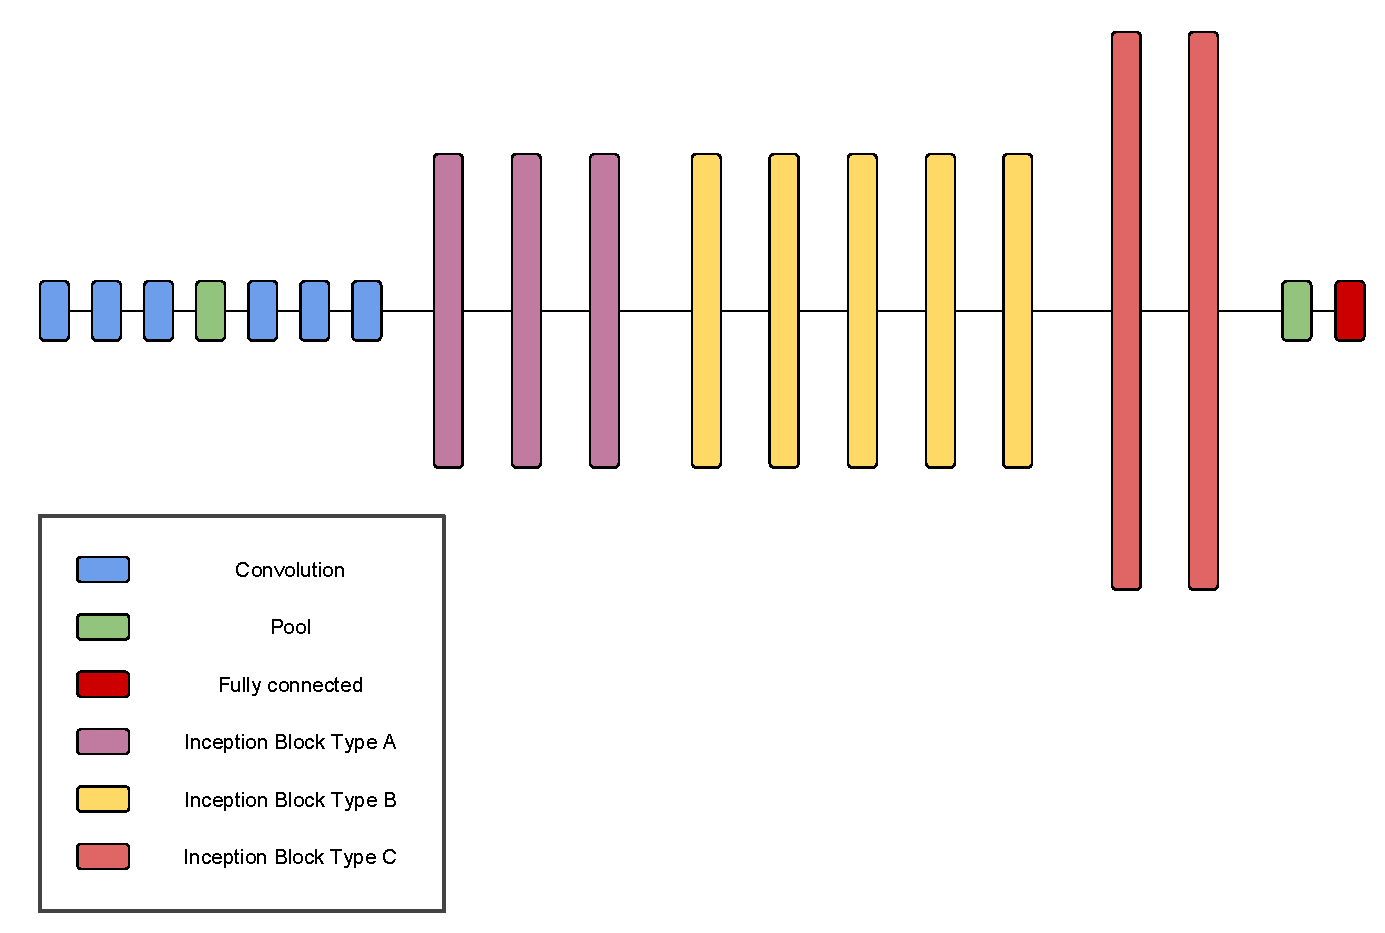
\includegraphics[width=18cm]{./figures/inception_schematic_fixed.pdf}
	\caption{Simplified diagram of Inception-v3 cropped at the fully connected layer.}
	\label{fig:inception}
\end{figure*}
\par



\begin{figure}
	\centering
		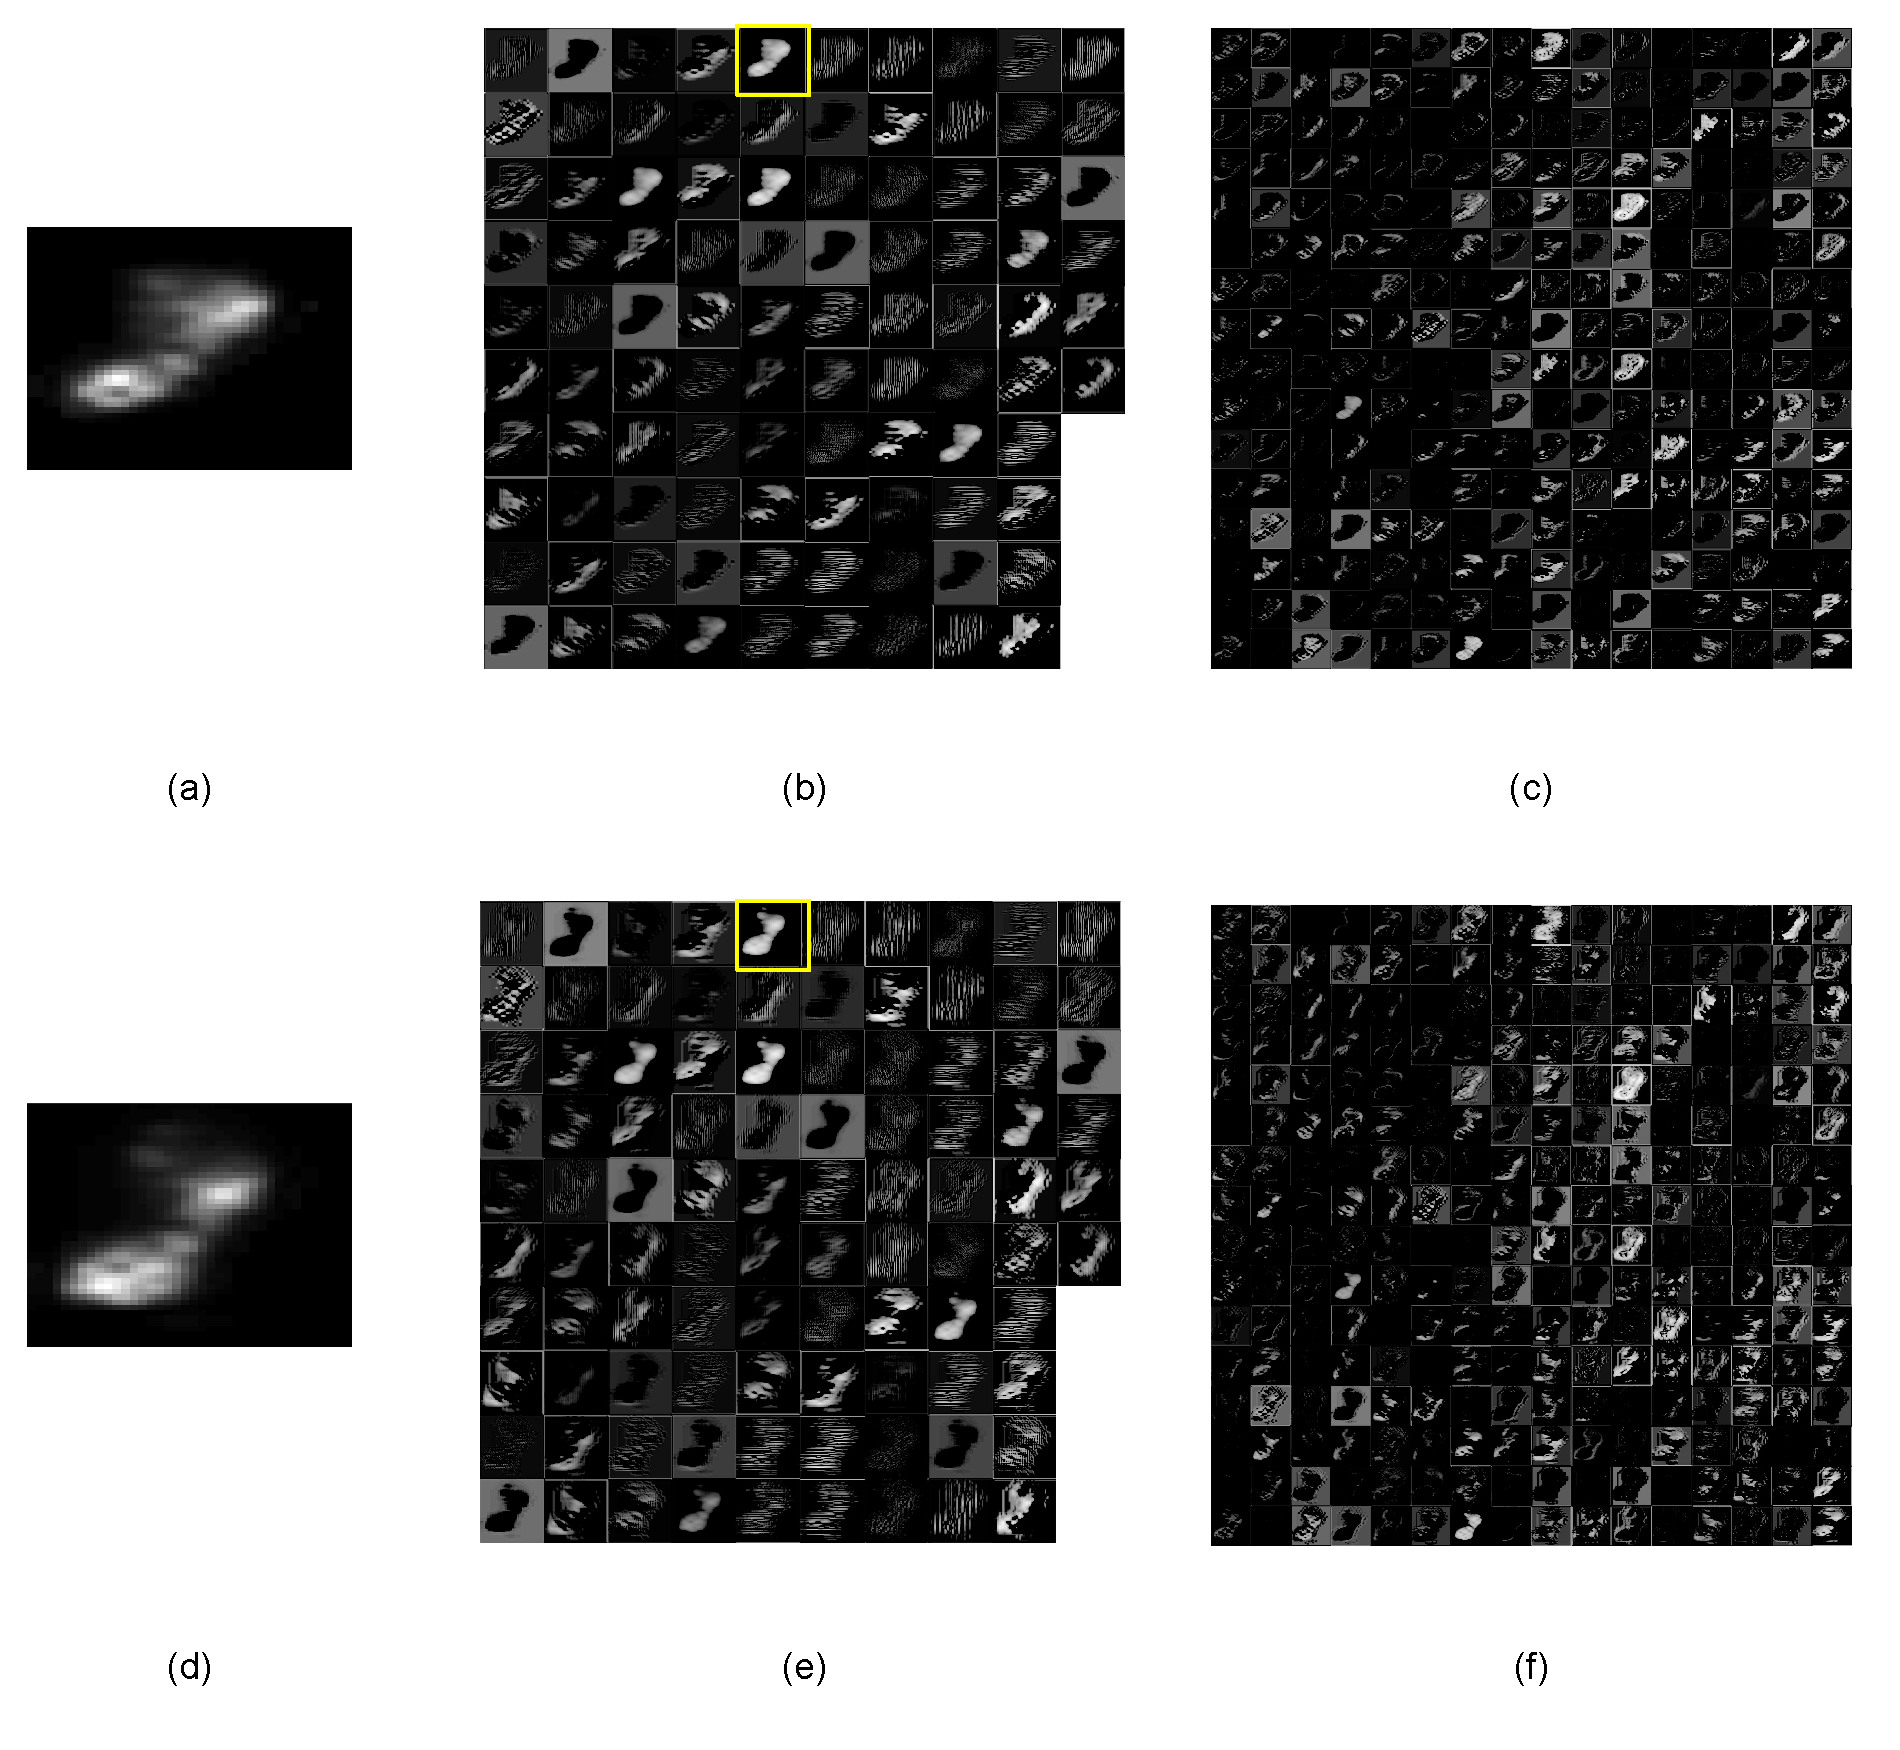
\includegraphics[width=9cm]{./figures/max_conv_vis.pdf}
	\caption{Visualization of information processing through different layers of AlexNet: (a) is the maximum frame and (d) the average frame of a single step sequence. (b) and (e) are the visualizations of the activation of the all filters in the first convolutional layer and (c) and (f) are visualizations from the second convolutional layer.    }
	\label{fig:max_conv_vis}
\end{figure}





